%! Author = brdvlami
%! Date = 30/04/2024

% Preamble
\documentclass[11pt]{article}

% Packages
\usepackage[english]{babel}
\usepackage{subfloat}
\usepackage{float}
\usepackage[style=ieee, backend=biber]{biblatex}
\addbibresource{abstract_bibliography.bib}
\renewcommand*{\bibfont}{\footnotesize}

\usepackage[small]{titlesec}
\titlespacing*{\section}{0pt}{3ex}{1ex}
\titlespacing*{\subsection}{0pt}{3ex}{0.5ex}
\titlespacing*{\subsubsection}{0pt}{3ex}{0.5ex}
\usepackage{multicol}
\usepackage{caption}
\captionsetup{font=footnotesize}
\usepackage[hyperfootnotes=true]{hyperref}
\usepackage{xcolor}
\hypersetup{
    colorlinks,
    linkcolor={black},
    citecolor={blue!50!black},
    urlcolor={blue!80!black}
}
%\setlength{\parindent}{0em}
\usepackage{geometry}
\geometry{
    a4paper,
    left=15mm,
    right=15mm,
    top=15mm,
    bottom=25mm,
}
\usepackage{graphicx}
\graphicspath{{./figures/}}

\newenvironment{Figure}
{\par\medskip\noindent\minipage{\linewidth}}
{\endminipage\par\medskip}


\newenvironment{Table}
{\par\medskip\noindent\minipage{\linewidth}}
{\endminipage\par\medskip}

\babelhyphenation[english]{Uni-Prot-KB}

% Document
\begin{document}

    \begingroup
    \centering
    \LARGE Unipept 6.0: Fast semi-exact peptide matching with a memory conservative index for UniProtKB\\[1em]
    \large Bram Devlaminck\\[2em]
    \endgroup

    \par\noindent\rule{\linewidth}{.5pt}
    \section*{Abstract}\label{sec:test-section}
    Unipept is an ecosystem developed for fast metaproteomics data-analyses.
    In the past few years Unipept has been optimized for tryptic peptides, with a slow workaround for peptides with missed cleavages.
    Unipept 6.0 introduces a new index structure which allows fast peptide matching for arbitrary peptides.
    This makes Unipept applicable in domains where trypsin is not the protease of choice, but also removes the performance introduced penalty when dealing with missed cleavages.
    All while outperforming competing tools.
    \par\noindent\rule{\linewidth}{.5pt}

    \begin{multicols}{2}
        \section{Introduction}\label{sec:introduction}
        Traditionally, the most used protease in the (meta)proteomics field is trypsin.
        Because of this, Unipept~\cite{unipept_desktop, unipept_api, unipept_4, unipept_orig, unipept_tutorial, unipept_web, unipept_cli, unipept_desktop_2} was specifically developed with this in mind.
        This resulted in the use of an index structure where the UniProtKB~\cite{UniprotKB} database is preprocessed by splitting every protein according to the cleavage pattern that trypsin creates.
        This also allows Unipept to precompute the LCA for every possible combination of matching tryptic peptides.
        This approach has proven its efficiency in the past few years, but also has its limitations.

        Trypsin will from time to time miss a cleavage position, this creates a so-called missed cleavage.
        Peptides with such missed cleavages will not be present in the current Unipept index, since Unipept assumes that there are no missed cleavages.
        To solve this problem, a solution was retro-fitted to handle these missed cleavages.
        When this option is selected, Unipept will scan the input peptide for these missed cleavage positions, split the peptide and perform separate lookups for every tryptic peptide.
        These results are intersected, which delivers a set of possible protein matches.
         Every protein in this set is brute-force scanned to ensure that the complete original peptide is present, and not only the separate tryptic fragments.
        Finally, the LCA of the found proteins is calculated on-the-fly.
        All these extra steps, including the on-the-fly calculation of the LCA has a significant impact on the performance when this option is enabled.

        A second disadvantage of the current Unipept index is the inability to process non-tryptic peptides.
        Similar to peptides with missed cleavages, these will not be present in the index, but there exists no workaround for this.

        This restriction has not been a significant problem since Unipept was originally created for the metaproteomics field, where trypsin is widely used.
        However, other fields such as the immunopeptidomics field frequently work with non-tryptic peptides.
        We aspire to broaden the use cases of Unipept, which requires a new search index with the following properties:

        \begin{enumerate}
            \item For every peptide (tryptic or non-tryptic), all matches in UniProtKB should be found.
            \item We need to be able to build the index for the full UniProtKB database with maximum memory usage around 1 to 2 TB of RAM\@.
            \item Search performance should be on par with the current Unipept index.
            \item The new index needs to be able to replace the current index, and facilitate all the current Unipept features.
        \end{enumerate}

        In short, we want an index that does not remove any of the current features, while remove the restriction that only tryptic peptides can efficiently be found by the current index.
        This also means that our new index will need to provide a way to equalize the amino acids isoleucine and leucine, as this is one of the current features.

        \section{Methods}\label{sec:methods}
        Our new index structure makes use of a suffix array.
        This suffix array can be build using the libdivsufsort~\cite{libdivsufsort} or libsais~\cite{libsais} library.
        Both provide a linear time algorithm with a $5n + O(1)$ memory complexity, where $n$ is the size of the text that needs to be indexed.

        \subsection{Sparse Suffix Arrays}
        While a complete suffix array delivers the best performance, the index itself is large.
        Since we are never interested in searching peptides that are less than 5 amino acids long\footnote{This is already a restriction in the current Unipept index, that has almost no real-world information loss associated with it because short peptides have thousands of matches, which makes the analysis results undetailed.}, we can make the suffix array sparse, which makes the resulting index smaller.
        This is accomplished by sampling the full suffix array, and only keeping every k-th suffix of the input text.
        This results in a sparse suffix array (SSA) which is only $\frac{1}{k}$th of the original suffix array size.

        \subsection{Equalizing Isoleucine and Leucine}
        Our solution to treat isoleucine and leucine as equal consists of 2 parts.
        Firstly, we don't index the original text, but a slightly modified version.
        We replace every occurrence of Leucine by Isoleucine, which essentially equalizes them during the construction of the suffix array.
        During the search, we perform the same translation on every peptide, and as a result we find every match with I and L equalized.
        We perform this search using the original, unmodified text.
        This is important, since we need this original text when we need to perform a search operation were we do not want to equalize I and L\@.
        In this case a second step is added.

        During this second step, we filter away the wrong matches from the first stage.
        This is achieved by checking every I and L location in the original, unmodified peptide with the matching amino acid in the original text.
        When these two characters are the same, there is indeed an exact match.
        A mismatch indicates that I and L were wrongfully equalized.
        Only these I and L locations have to be checked since the suffix array search already ensures that all other characters match in the original text.

        \subsection{Analyses}
        Our solution performs the functional and taxonomic analysis at runtime.
        While it would be advantageous to precompute this, the suffix array and text do not contain enough information to do this.
        This is a trade-off we made during development between max memory usage and speed.
        In practice, this is not a big limitation.

        \section{Results}\label{sec:results}
        Three main aspects are considered during testing.
        The memory usage and speed during building, the resulting index size while hosting and search performance.

        \subsection{Building the Index}
        Building the suffix array for the complete UniProtKB database requires around 735 GB of RAM and 5 hours of computing time using the libdivsufsort library.
        Because of the high-memory needs, we use the HPC of Ghent University, where the high-memory cluster has 16 nodes with each 2\times 64-core AMD EPYC 7773X (Milan-X @ 2.2 GHz) and 940 GB of RAM\@.
        We use one core of a single node since the construction phase is single threaded.
        The resulting full suffix array is around 700 GB large (+ another 88 GB for the text).
        Our goal is to host this new index on Unipept servers, which have around 0.5 TB of available memory.
        To make this possible, we immediately perform a sampling phase with sparseness factor $k = 3$ at the end of the construction process on the HPC\@.
        This results in a search index size of $\frac{700}{3} + 88 \approx 322$ GB\@.
        Next to this search index Unipept needs some extra information (such as the UniProt accession number, NCBI taxon ID and functional annotations per protein).
        This results in another 25 GB of needed RAM\@.

        \begin{Figure}
            \centering
            \resizebox{\textwidth}{!}{
            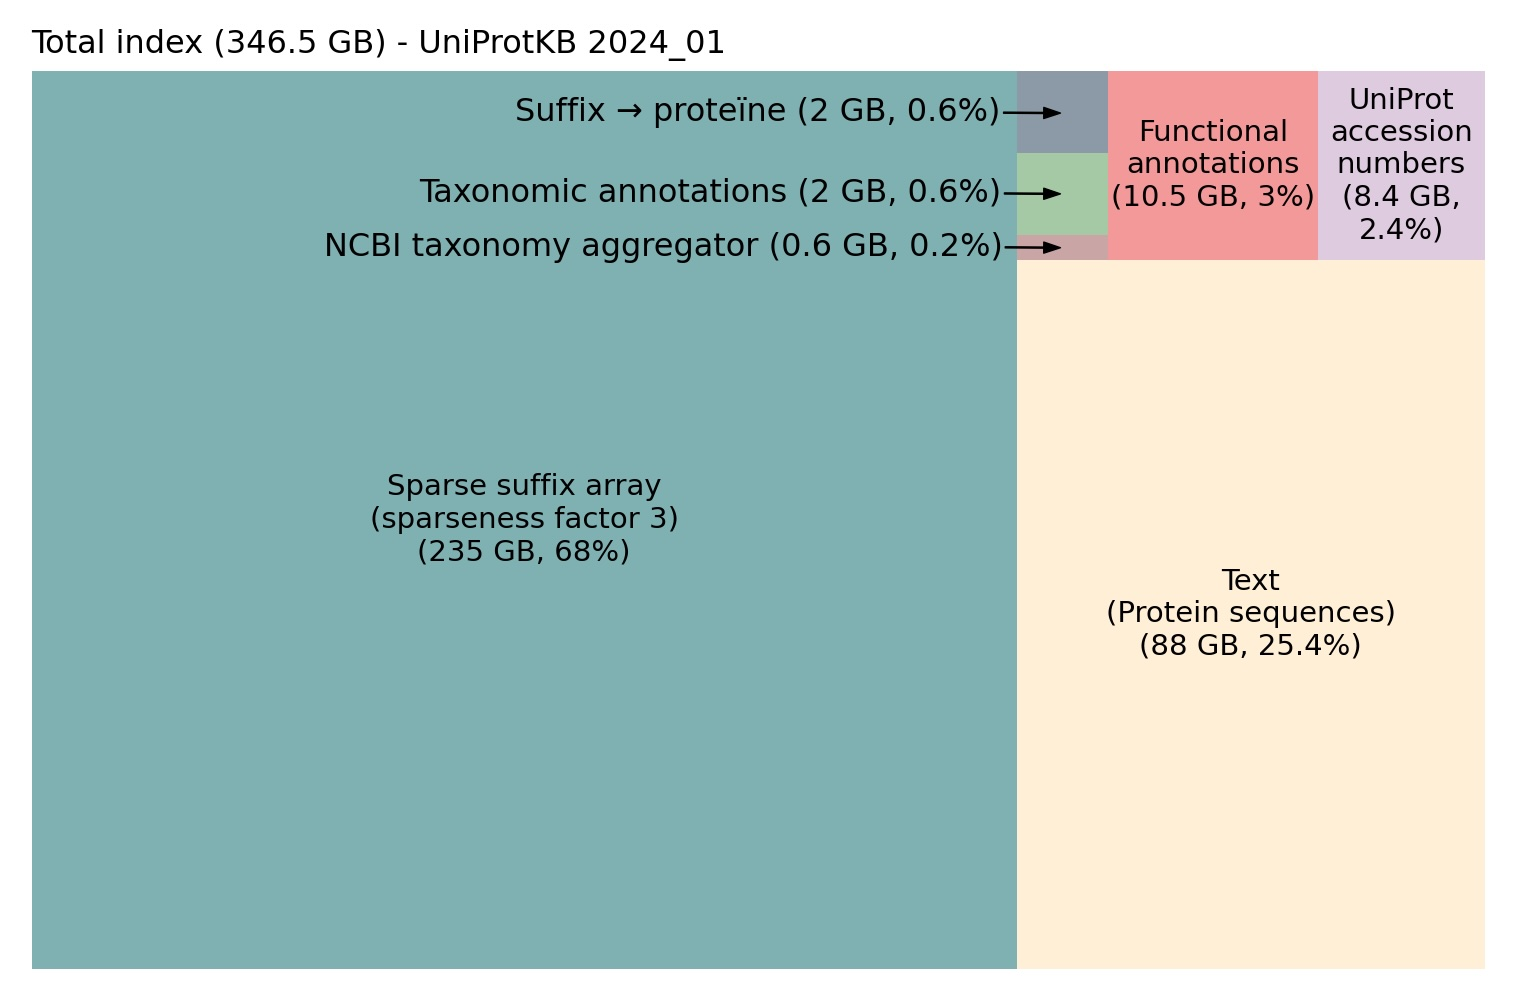
\includegraphics{uniprot_memory_treemap}
            }
            \captionof{figure}{Visualisation of the size of each part of the new Unipept index for UniProtKB 2024\_01.}
            \label{fig:uniprot_memory_treemap}
        \end{Figure}

        \subsection{Querying the index}
        To evaluate the performance we use 6 files with each around 25\thinspace000 peptides.
        These are samples from the SIHUMIx experiment, where trypsin is used as a protease.
        This means that as well as tryptic peptides, there are also peptides with naturally occurring missed cleavages present.
        Figure~\ref{fig:new_vs_old_unipept} shows the execution time for both the new and old unipept index.
        To make the comparison as fair as possible the \textit{filter duplicate peptides} setting is turned off, and \textit{advanced missed cleavage handling} is turned on.
        This way the old unipept index also searches for all entries (including duplicates), while still finding matches for peptides with missed cleavages.
        Note that the old Unipept index will not find peptides that are created by another protease, while this makes no difference for the new index.
        \begin{Figure}
            \centering
            \resizebox{\textwidth}{!}{
                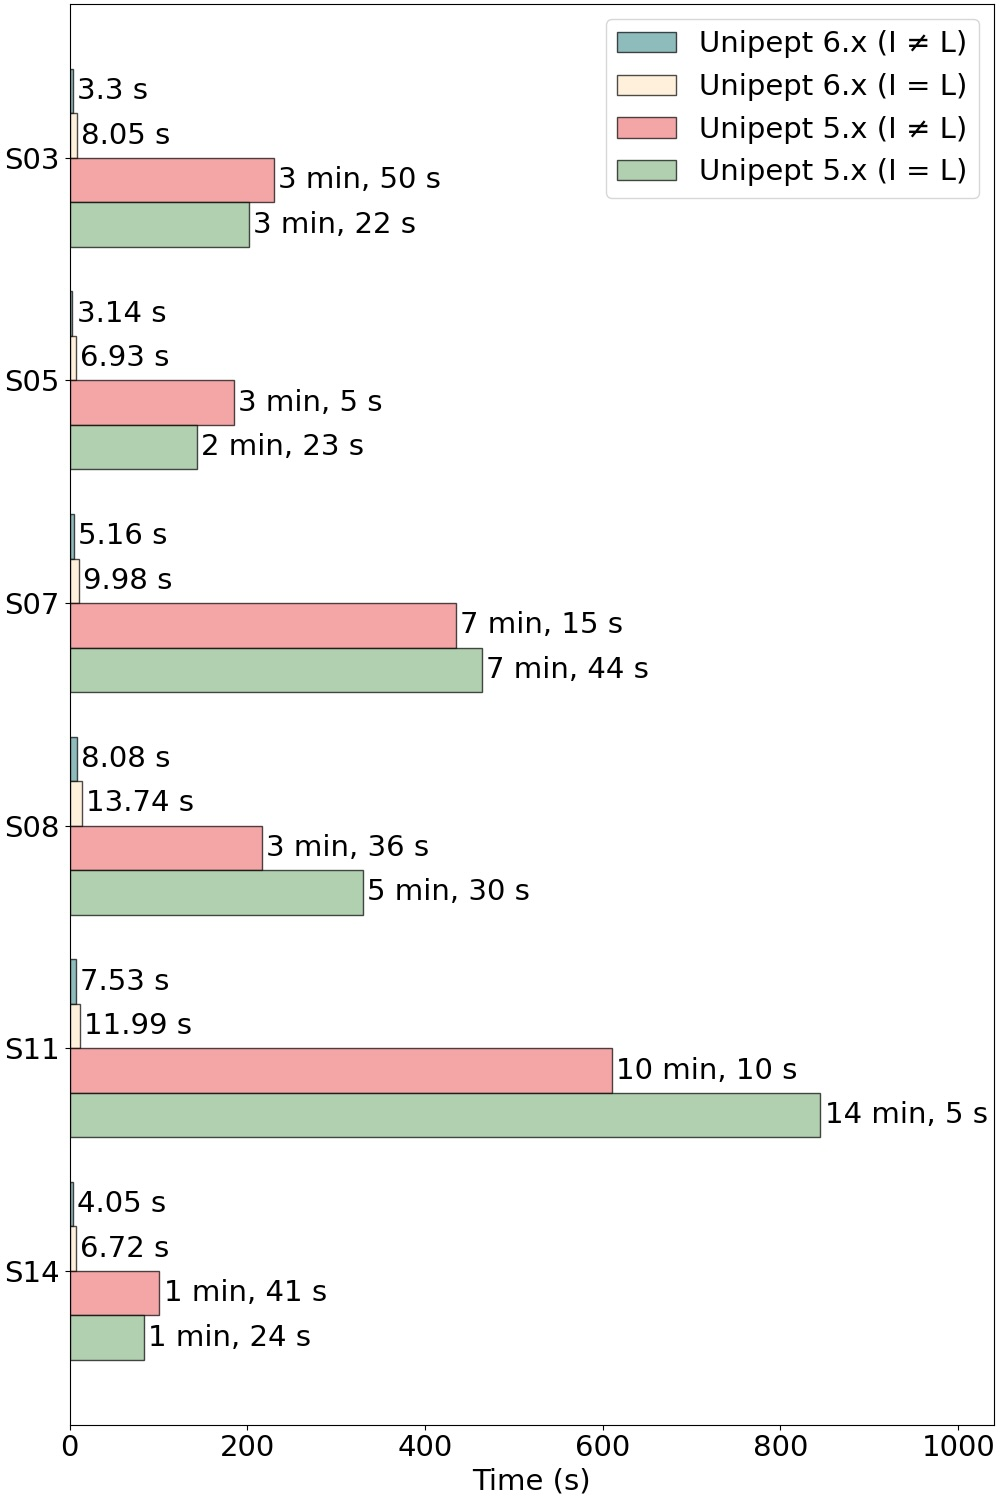
\includegraphics{new_vs_old_unipept}
            }
            \captionof{figure}{Execution time for the new and old Unipept index while searching different SIHUMIx samples. Each sample consists of approximately 25\thinspace000 peptides. The old Unipept index searches with the \textit{filter duplicate peptides} setting turned off, and \textit{advanced missed cleavage handling} turned on. This way both indices search all peptides (included duplicates), and missed cleavages are handled by both.}
            \label{fig:new_vs_old_unipept}
        \end{Figure}
        When we compare the new index to the old index when only searching for tryptic peptides, we notice that the new index is around 1.5 times slower.
        This is mainly the impact from the analyses that has to be performed during search, instead of just being able to retrieve it.
        Furthermore, it is clearly visible that the extra filtering step has a performance impact on the big peptide files.
        This effect was not clearly visible in Figure~\ref{fig:new_vs_old_unipept}, where the reverse seems to be visible.
        However, this reverse effect is because searching with I = L finds more matches, which requires more output to be serialized to JSON\@.
        In the bigger tests the extra time spend during search compensates for this. % TODO: figure about tryptic search

        \section{Comparison}\label{sec:comparison}
        To compare our new index we need to take multiple aspects in to account.
        Tools such as the Uniprot peptide search tool~\cite{uniprot_search_site, uniprot_search_paper}, the Expasy ScanProsite tool~\cite{scanprosite} and Unipept at the moment all have the possibility to find matches in the UniProtKB database.
        There are some major differences though.

        Feature wise, the UniProt Peptide Search tool is identical to the new suffix array index developed for Unipept.
        They can both find all matches in UniProtKB, and have the option to equalize I and L\@.
        The only difference is the performance.
        Searching one peptide in the SA only takes a few milliseconds, while the UniProt tool takes a few seconds up to multiple minutes.

        Expasy ScanProsite tool takes another approach.
        They provide a wide range of options for inexact matching.
        They call this motives, ant these are comparable to regular expressions where the user can use wildcards, character classes and even negations.
        The other major difference is that this tool does not use the whole UniProtKB database.
        Only the proteins that are part of a reference genome are indexed, which means that less matches are found.

        The last major tool we compare with is the current Unipept index.
        As described in the introduction we wanted to keep all the current features of Unipept, with the addition of removing the restriction where Unipept can only quickly find tryptic peptides (or with a performance penalty also tryptic peptides with missed cleavages).
        This means that every non-tryptic peptide will result in 0 matches in the old index, while the new index will find all matches that are in UniProtKB\@.
        Table~\ref{tab:tool_comparison} gives a small overview of the described differences between the tools.

        \begin{Table}
            \centering
            \resizebox{\textwidth}{!}{
                \begin{tabular}{ l l l l l }
                    & SSA    & UPS          & ESP        & UP             \\
                    \hline\hline
                    Used Prot.   & all    & all          & ref. prot. & all            \\
                    Approx Match & [IL]   & [IL]         & flexible   & [IL]           \\
                    time         & $<$ 5 ms & 1 s - 20 min & 5 min      & $<$ 5 ms         \\
                    Valid pept.  & all    & all          & all        & $\sim$ tryptic \\
                    \hline
                \end{tabular}
            }
            \captionof{table}{Comparison of the new suffix array (SA), UniProt Peptide Search (UPS) tool, Expasy ScanProSite (ESP) tool and the current Unipept (UP) index.}
            \label{tab:tool_comparison}
        \end{Table}

        \section{Conclusion}\label{sec:discussion}
        With a new core index structure at the heart of Unipept we have broadened Unipept's possible use cases.
        The new index structure makes searching peptides with missed cleavages around 10 to 100 times faster.
        While adding the possibility to search arbitrary peptides, regardless of the used protease.
        From our testing, Unipept greatly outperforms its closest competitors at finding all occurrences for an arbitrary peptide longer than 2 amino acids in UniProtKB\@.
        The disadvantage of this new index is that searching tryptic peptides is slightly slower than before.
        This slowdown is created by the analyses that has to be performed during search itself, while this could all be precalculated once in the old index.

        Another advantage of the new index is that there are no extra steps required to retrieve the NCBI taxon ID for each matched protein.
        The current index requires extra steps to retrieve this, with a significant impact on the performance.
        This restriction creates a bottleneck in the new Peptonizer2000 tool.

        \section{Future work}
        The new index solves the pre-set targets, but still leaves room for improvement in several areas.

        A significant part of the current computation time is invested in performing the taxonomic and functional analyses.
        Modifying the new index to support the pre-calculation of these analyses, while still maintaining a peak memory usage which is manageable would drastically improve the performance.

        The index size could be reduced even more by making the text and suffix array even more compact.
        Both of these structures don't utilize all bits from the allocated bytes.
        The suffix array only needs 37 of the 64 bits used by every entry, while the text only needs 5 bits out of each byte per character.
        This would reduce the total index size from 364 GB to around 225 GB\@.
        However, this would introduce extra steps to decode every access to any of these data structures.
        This could introduce non-negligible performance penalty.

        Lastly, Unipept does not perform any form of inexact matching, except for I and L\@.
        Introducing inexact matching into Unipept could allow us to deal with small mutations or read-errors introduced by a mass spectrometer.
        \printbibliography
    \end{multicols}




\end{document}